\section{Event Selections}
\label{sec:EventSelections}
%\todo[inline]{Give a brief overview of the three selections, even if they're unchanged from previous note, along with cut tables.}
%focus on changes with respect to the previous selection
%(Kate+Sophie

%\subsection{Preselections}

%The preselections employed are unchanged from the previous analysis and defined below.

This section describes the neutrino event selections in this analysis. These are the the electron (1e0p0$\pi$, 1eNp0$\pi$) and muon (1$\mu$0pX$\pi$) neutrino selections.  These selections are in large part unchanged from the run 1-3 analysis~\cite{PELEEpaper}.  In particular the muon neutrino selection is identical.  The electron neutrino selection adds selection cuts related to the CRT on top of the previous selections to improve cosmic rejection, and further description is given in~\ref{CRTsection}. Cut tables are included in Appendix A.  Validation of the selection over the full run 1-5 data set is described in Section~\ref{Validation}.  

\subsection{Cosmic Ray Tagger (CRT)}
\label{sec:CRTsection}

The purpose of the CRT is to reduce cosmic background in the analysis. The muon neutrino selections for Run 3 - Run 5 data already uses CRT data for cosmic reduction~\cite{PELEEpaper,PELEEtechnote}. Now, CRT data will be used for electron neutrino selections for Run 3 - Run 5 data. 

The two main concepts the CRT relies on for cosmic reduction are vetoing cosmic rays and tagging them based on distance. The variables used for these CRT rejection cuts, as defined in~\cite{PELEEtechnote}, are:\\
\\
\textbf{crtveto}: Boolean variable checking if the event passes the CRT veto.\\
\textbf{crthitpe}: How many photoelectrons (PEs) were recorded by the CRT system.\\
\textbf{\_closestNuCosmicDist}: 3D distance, measured in centimeters, between the reconstructed neutrino vertex and the closest CRT-tagged cosmic track.\\
\\
The CRT selection cuts that are applied to electron and muon neutrino selections in the analysis, defined by~\cite{PELEEtechnote}, are as follows:

\begin{center}
    crtveto != 1  or crthitpe \(<\) 100 
\end{center}
\begin{center}
    \_closestNuCosmicDist \(>\) 5
\end{center}

Figures~\ref{fig:1eNp_preselection},~\ref{fig:1eNp_loosecuts},~\ref{fig:1e0p_preselection}, and~\ref{fig:1e0p_loosecuts} show the effect of these CRT cuts when plotting events as a function of reconstructed energy. In these these and following figures in this note, distributions are shown as stacked histograms, with colors indicating the event type. Hatched histograms labeled "EXT" correspond to the background expectation from beam-off data. Error bands correspond to the uncorrelated errors in each bin, including statistical and systematic uncertainties. Black solid lines labeled "MC+EXT" correspond to the total predicted event counts from MC simulated signal events and EXT background. If sideband constraints are included in a plot, the "MC+EXT" line will include sideband corrections and therefore may not correspond to the total bin count of the stacked histograms.

\begin{figure}[H] \centering
    \begin{subfigure}[t]{0.45\linewidth}
        \includegraphics[width=\linewidth]{technote/EventSelections/FiguresCRT/run5_Np_presel.png}
        \caption{Reconstructed Neutrino Energy without CRT cuts}
    \end{subfigure}%
    \hspace{0.45cm}%
    \begin{subfigure}[t]{0.45\linewidth}
        \includegraphics[width=\linewidth]{technote/EventSelections/FiguresCRT/run5_Np_presel_crt.png}%
        \caption{Reconstructed Neutrino Energy with CRT cuts}
    \end{subfigure}%
    \caption{Comparison of reconstructed neutrino energy for Run 5 1eNp0$\pi$ preselection, with and without the application of CRT cuts to the event selection.}
    \label{fig:1eNp_preselection}
\end{figure}

\begin{figure}[H] \centering
    \begin{subfigure}[t]{0.45\linewidth}
        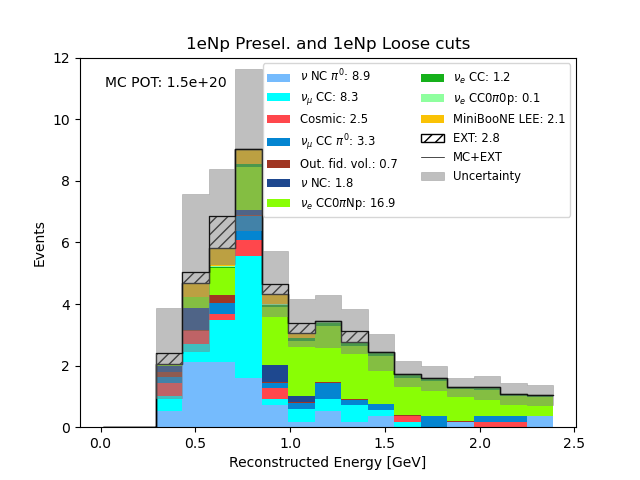
\includegraphics[width=\linewidth]{technote/EventSelections/FiguresCRT/NPloose.png}
        \caption{Reconstructed Neutrino Energy without CRT cuts}
    \end{subfigure}%
    \hspace{0.45cm}%
    \begin{subfigure}[t]{0.45\linewidth}
        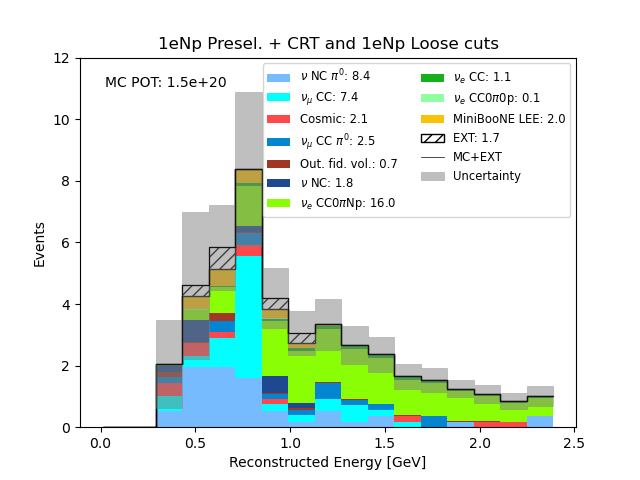
\includegraphics[width=\linewidth]{technote/EventSelections/FiguresCRT/NPlooseCRT.png}%
        \caption{Reconstructed Neutrino Energy with CRT cuts}
    \end{subfigure}%
    \caption{Comparison of reconstructed neutrino energy for Run 5 1eNp0$\pi$ loose box cuts, with and without the application of CRT cuts to the event selection.}
    \label{fig:1eNp_loosecuts}
\end{figure}

\begin{figure}[H] \centering
    \begin{subfigure}[t]{0.45\linewidth}
        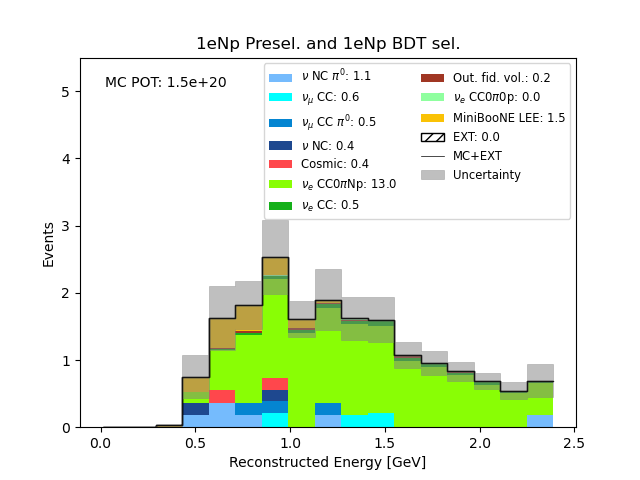
\includegraphics[width=\linewidth]{technote/EventSelections/FiguresCRT/NPBDT.png}
        \caption{Reconstructed Neutrino Energy without CRT cuts}
    \end{subfigure}%
    \hspace{0.45cm}%
    \begin{subfigure}[t]{0.45\linewidth}
        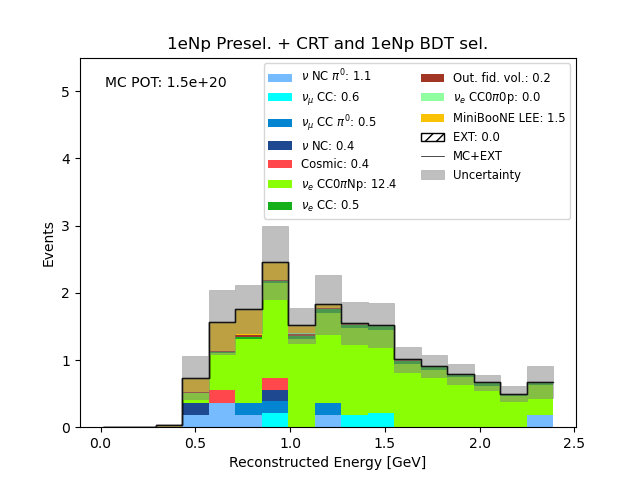
\includegraphics[width=\linewidth]{technote/EventSelections/FiguresCRT/NPBDTCRT.png}%
        \caption{Reconstructed Neutrino Energy with CRT cuts}
    \end{subfigure}%
    \caption{Comparison of reconstructed neutrino energy for Run 5 1eNp0$\pi$ BDT selection, with and without the application of CRT cuts.}
    \label{fig:1eNp_BDT}
\end{figure}

\begin{figure}[H] \centering
    \begin{subfigure}[t]{0.45\linewidth}
        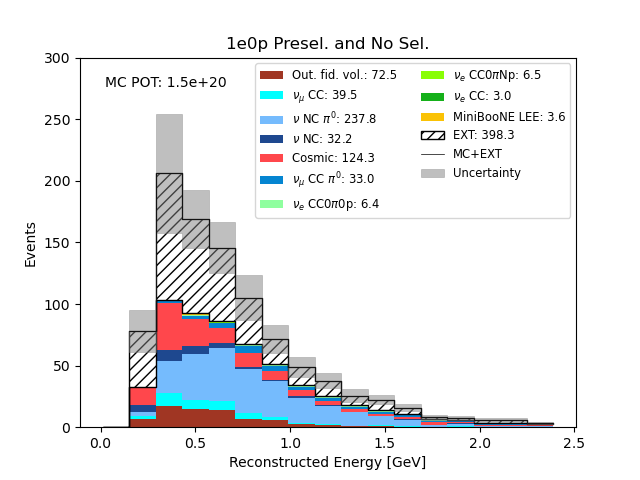
\includegraphics[width=\linewidth]{technote/EventSelections/FiguresCRT/0Ppresel.png}
        \caption{Reconstructed Neutrino Energy without CRT cuts}
    \end{subfigure}%
    \hspace{0.45cm}%
    \begin{subfigure}[t]{0.45\linewidth}
        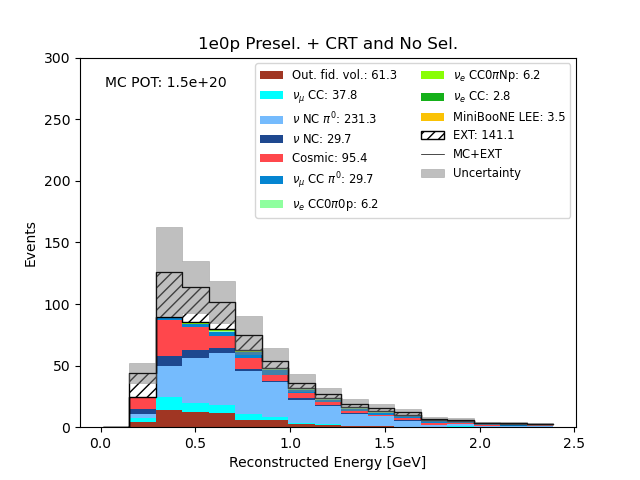
\includegraphics[width=\linewidth]{technote/EventSelections/FiguresCRT/0PpreselCRT.png}%
        \caption{Reconstructed Neutrino Energy with CRT cuts}
    \end{subfigure}%
    \caption{Comparison of reconstructed neutrino energy for Run 5 1e0p0$\pi$ preselection, with and without the application of CRT cuts to the event selection.}
    \label{fig:1e0p_preselection}
\end{figure}

\begin{figure}[H] \centering
    \begin{subfigure}[t]{0.45\linewidth}
        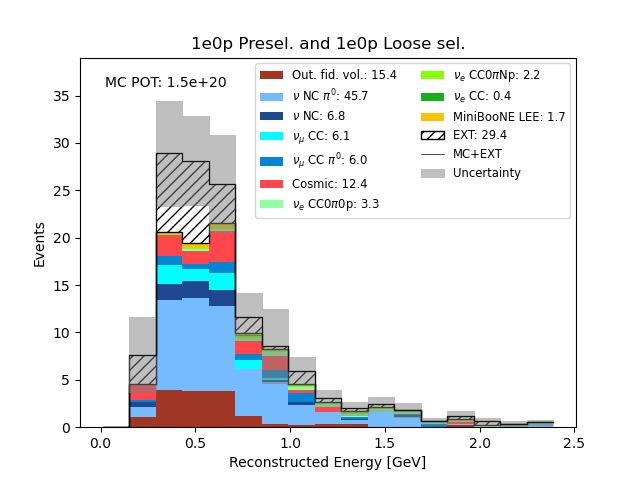
\includegraphics[width=\linewidth]{technote/EventSelections/FiguresCRT/0Ploose.png}
        \caption{Reconstructed Neutrino Energy without CRT cuts}
    \end{subfigure}%
    \hspace{0.45cm}%
    \begin{subfigure}[t]{0.45\linewidth}
        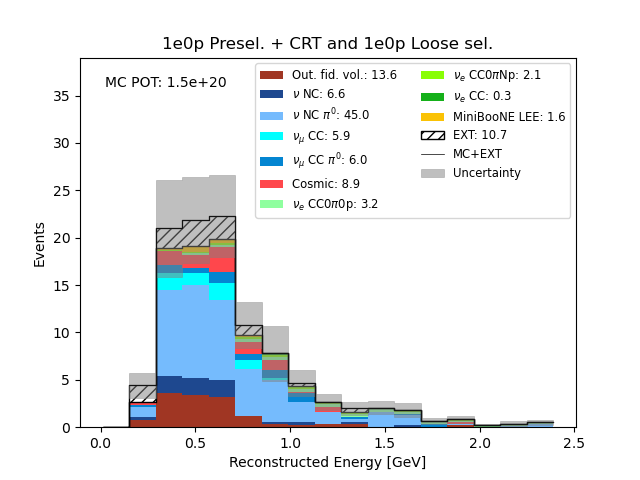
\includegraphics[width=\linewidth]{technote/EventSelections/FiguresCRT/0PlooseCRT.png}%
        \caption{Reconstructed Neutrino Energy with CRT cuts}
    \end{subfigure}%
    \caption{Comparison of reconstructed neutrino energy for Run 5 1e0p0$\pi$ loose box cuts, with and without the application of CRT cuts to the event selection.}
    \label{fig:1e0p_loosecuts}
\end{figure}

\begin{figure}[H] \centering
    \begin{subfigure}[t]{0.45\linewidth}
        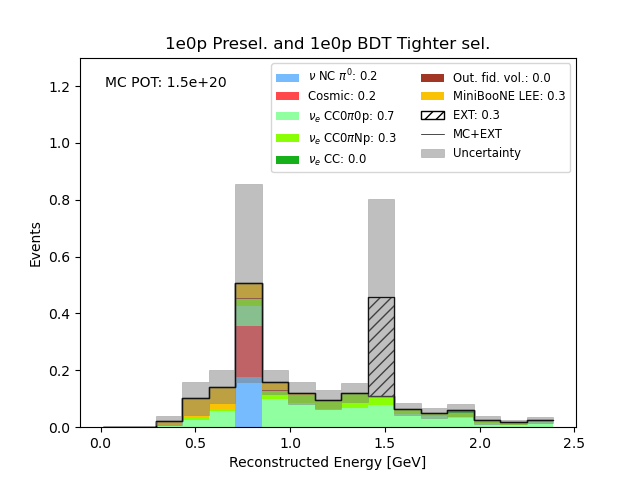
\includegraphics[width=\linewidth]{technote/EventSelections/FiguresCRT/0PBDT.png}
        \caption{Reconstructed Neutrino Energy without CRT cuts}
    \end{subfigure}%
    \hspace{0.45cm}%
    \begin{subfigure}[t]{0.45\linewidth}
        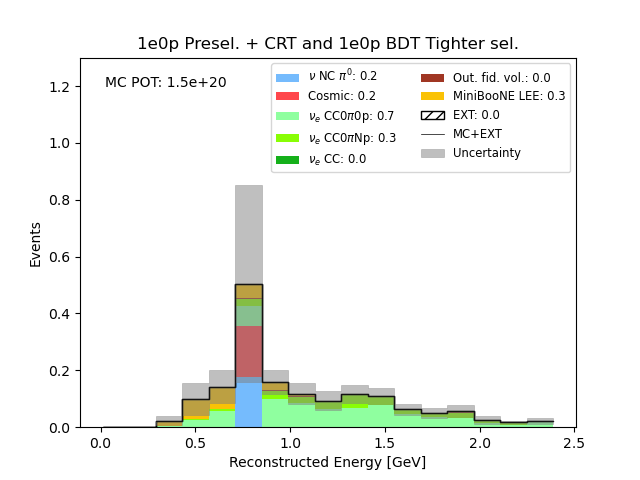
\includegraphics[width=\linewidth]{technote/EventSelections/FiguresCRT/0PBDTCRT.png}%
        \caption{Reconstructed Neutrino Energy with CRT cuts}
    \end{subfigure}%
    \caption{Comparison of reconstructed neutrino energy for Run 5 1e0p0$\pi$ BDT selection, with and without the application of CRT cuts.}
    \label{fig:1eNp_BDT}
\end{figure}

\begin{table} [h!]
    \centering
    \begin{tabular}{| c | c | c |}
         \hline
         \textbf{Selection} & \textbf{EXT Survival Rate} & \textbf{Nue Efficiency} \\  [0.75ex]
         \hline
         1eNp0$\pi$ Preselection & 35.1\% & 94.8\% \\ 
         \hline
         1eNp0$\pi$ Loose Box Cuts & 60.7\% & 94.5\% \\ 
         \hline
         1eNp0$\pi$ BDT & N/A & 95.6\% \\ 
         \hline
         1e0p0$\pi$ Preselection & 35.4\% & 95.6\% \\ 
         \hline
         1e0p0$\pi$ Loose Box Cuts & 36.4\% & 94.9\% \\ 
         \hline
         1e0p0$\pi$ BDT & 0\% & 100\% \\ 
         \hline 
    \end{tabular}
    \caption{EXT survival rates and electron neutrino efficiency rates for given event selections.}
    \label{tab:EXT_survival_table}
\end{table}

As the CRT is a new piece of hardware that has to date only been used in Run 3, it was necessary to check if its operations were stable in time. This analysis was done by looking at the EXT survival vs. `run number' for run periods 3, 4b, 4c, 4d, and 5 with and without CRT cuts. This is done by taking a ratio of EXT with CRT cuts and EXT without CRT cuts to acquire the rate at which cosmic events survive the CRT cuts. 

\begin{figure}[H]
 \centering
    \begin{subfigure}[t]{0.31\linewidth}
        \includegraphics[width=\linewidth]{technote/EventSelections/FiguresCRT/run5_CRT1.png}
        \caption{EXT vs. `run' with CRT cuts}
    \end{subfigure}%
    \hspace{0.3cm}%
    \begin{subfigure}[t]{0.31\linewidth}
        \includegraphics[width=\linewidth]{technote/EventSelections/FiguresCRT/run5_noCRT1.png}%
        \caption{EXT vs. `run' without CRT cuts}
    \end{subfigure}%
    \hspace{0.3cm}%
    \begin{subfigure}[t]{0.32\linewidth}
        \includegraphics[width=\linewidth]{technote/EventSelections/FiguresCRT/run5fortalk.png}%
        \caption{Survival rate of EXT events}
    \end{subfigure}
    \caption{Analysis of EXT events vs. run number with overall event selection of `nslice==1', then with (a) and without (b) CRT cuts. The applied CRT cut here is `crtveto != 1'. Figure (c) shows the ratio of how many EXT events pass through the CRT cuts, or the survival rate. }
    \label{fig:EXT_survival_run5}
\end{figure}

Figure~\ref{fig:EXT_survival_run5} shows the rate at which EXT events pass the CRT cuts. To acquire the rejection ratio instead of the survival ratio, one can subtract the survival rate from 1. Figure~\ref{fig:EXT_survival_run5} shows the specific case of finding the survival rate using Run 5 beam off data, with the selection of `nslice == 1', and the CRT cut `crtveto != 1'. 
This analysis was done for various CRT selection cuts as well as various neutrino selections. We examine each of the CRT variables individually, the veto variables separately, and then the entire CRT selection. For each of these CRT configurations, we examine the event selections of `nslice == 1', as well as electron neutrino preselection and muon neutrino preselection. 
Figure~\ref{fig:EXT_survival_allruns} uses the same selection as Figure~\ref{fig:EXT_survival_run5} and shows the EXT survival rate plots for run periods 3, 4b-d, and 5.

\begin{figure}[H]
 \centering
    \begin{subfigure}[t]{0.3\linewidth}
        \includegraphics[width=\linewidth]{technote/EventSelections/FiguresCRT/run3_rationew.png}
        \caption{Survival rate of EXT events for Run 3}
    \end{subfigure}%
    \hspace{0.3cm}%
    \begin{subfigure}[t]{0.3\linewidth}
        \includegraphics[width=\linewidth]{technote/EventSelections/FiguresCRT/run4b_ratio1.png}%
        \caption{Survival rate of EXT events for Run 4b}
    \end{subfigure}%
    \hspace{0.3cm}%
    \begin{subfigure}[t]{0.3\linewidth}
        \includegraphics[width=\linewidth]{technote/EventSelections/FiguresCRT/run4cfortalk.png}%
        \caption{Survival rate of EXT events for Run 4c}
    \end{subfigure}
    \hspace{0.3cm}%
    \begin{subfigure}[t]{0.3\linewidth}
        \includegraphics[width=\linewidth]{technote/EventSelections/FiguresCRT/run4dfortalk.png}%
        \caption{Survival rate of EXT events for Run 4d}
    \end{subfigure}
    \hspace{0.3cm}%
    \begin{subfigure}[t]{0.3\linewidth}
        \includegraphics[width=\linewidth]{technote/EventSelections/FiguresCRT/run5fortalk.png}%
        \caption{Survival rate of EXT events for Run 5}
    \end{subfigure}
    \caption{EXT event survival rates for runs 3, 4b-d, and 5. }
    \label{fig:EXT_survival_allruns}
\end{figure}

It is clear from Figure~\ref{fig:EXT_survival_allruns}, and this trend holds for the different CRT cut configurations and event selections, that the survival rate is not constant across these run periods. Regions of particular interest include the beginning of Run 3, the step up in Run 4b, and the sharp decrease in survival rate from Run 4c to Run 4d. This stability check revealed inconsistencies in the production of the beam off files in regards to the CRT variables. CRT-TPC merging was not performed correctly for some of the data sets and this led to this inconsistency~\cite{Herbspresentation}.  %add this citation

Once the re-merging is done, we will once again check the time dependence and stability of EXT survival for various selections. Following these stability checks, the full analysis of 1eNp0$\pi$ and 1e0p0$\pi$ event selections can be done with the CRT included in selection cuts.

\subsection{Selection validation}
\label{sec:selvalid}

The event selections employed in this note to generate the 1e0p, 1eNp signals channels, and $\nu_{\mu}$ and $\pi^0$ sidebands, are unchanged from those of the previous analysis. \todo{Update if we include CRT cuts/0 pion cuts}. However MC simulation samples and the framework employed to produce data/MC simulation comparisons have been updated and therefore require validation. Section~\ref{sec:compprevframework} contains a number of comparisons between the new and old analysis frameworks, and a wide variety of variables are compared to MC simulation after applying the preselections in Appendix~\ref{appendix:PreselectionValidation}. Additionally, comparisons between data and MC simulation for many combinations of selections and variables are shown for a number of sidebands in Section~\ref{sec:sidebands}

\subsubsection{Comparison with Previous Framework}
\label{sec:compprevframework}

In order to check the consistency with the previous analysis, a range of checks were performed using various sample/event selection combinations. Three copies of each distribution were produced using three different versions of the code:
%
\begin{enumerate}
    \item The old analysis code, with the old data loading module (\verb|load_data_run123.py|) and the old plotting module (\verb|plotter.py|).
    \item The new data loading module (\verb|data_loading.py|), with the old plotting module.
    \item The new data loading and plotting modules.
\end{enumerate}
%
The outputs of these three module combinations are then compared, an example of this comparison is shown in Figures~\ref{fig:distvalidation_1e0p},~\ref{fig:distvalidation_1eNp}, and~\ref{fig:distvalidation_NuMu}\footnote{The minor discrepancy in the EXT in these plots can be explained by different approaches to the POT weighting when multiple runs are used. The new framework applies a POT scaling to the events from each individual run before combining them, whereas the old codebase would combine the runs together and then weight them.}.
%
\begin{figure}[H]
 \centering
    \begin{subfigure}[t]{0.32\linewidth}
        \includegraphics[width=\linewidth]{technote/EventSelections/Figures/Run123_1e0p_RecoEnergy_Old.png}
        \caption{Using the old data loading and plotting modules.}
    \end{subfigure}%
    \hspace{0.3cm}%
    \begin{subfigure}[t]{0.32\linewidth}
        \includegraphics[width=\linewidth]{technote/EventSelections/Figures/Run123_1e0p_RecoEnergy_Chris.png}%
        \caption{Using the new data loading with the old plotting module.}
    \end{subfigure}%
    \hspace{0.3cm}%
    \begin{subfigure}[t]{0.31\linewidth}
        \includegraphics[width=\linewidth]{technote/EventSelections/Figures/Run123_1e0p_RecoEnergy_Alex.png}
        \caption{Using the new data loading and plotting modules.}
    \end{subfigure}% 
    \caption{Three copies of the reconstructed neutrino energy distribution produced with the three different module combinations for the purpose of software validation, using the full 1e0p event selection.}
    \label{fig:distvalidation_1e0p}
\end{figure}

\begin{figure}[H]
 \centering
    \begin{subfigure}[t]{0.32\linewidth}
        \includegraphics[width=\linewidth]{technote/EventSelections/Figures/Run123_1eNp_RecoEnergy_Old.png}
        \caption{Using the old data loading and plotting modules.}
    \end{subfigure}%
    \hspace{0.3cm}%
    \begin{subfigure}[t]{0.32\linewidth}
        \includegraphics[width=\linewidth]{technote/EventSelections/Figures/Run123_1eNp_RecoEnergy_Chris.png}%
        \caption{Using the new data loading with the old plotting module.}
    \end{subfigure}%
    \hspace{0.3cm}%
    \begin{subfigure}[t]{0.31\linewidth}
        \includegraphics[width=\linewidth]{technote/EventSelections/Figures/Run123_1eNp_RecoEnergy_Alex.png}
        \caption{Using the new data loading and plotting modules.}
    \end{subfigure}% 
    \caption{Three copies of the reconstructed neutrino energy distribution produced with the three different module combinations for the purpose of software validation, using the full 1eNp event selection.}
    \label{fig:distvalidation_1eNp}
\end{figure}

\begin{figure}[H]
 \centering
    \begin{subfigure}[t]{0.32\linewidth}
        \includegraphics[width=\linewidth]{technote/EventSelections/Figures/Run123_NuMu_RecoEnergy_Old.png}
        \caption{Using the old data loading and plotting modules.}
    \end{subfigure}%
    \hspace{0.3cm}%
    \begin{subfigure}[t]{0.32\linewidth}
        \includegraphics[width=\linewidth]{technote/EventSelections/Figures/Run123_NuMu_RecoEnergy_Alex.png}%
        \caption{Using the new data loading with the old plotting module.}
    \end{subfigure}%
    \hspace{0.3cm}%
    \begin{subfigure}[t]{0.31\linewidth}
        \includegraphics[width=\linewidth]{technote/EventSelections/Figures/Run123_NuMu_RecoEnergy_Old.png}
        \caption{Using the new data loading and plotting modules.}
    \end{subfigure}% 
    \caption{Three copies of the reconstructed neutrino energy distribution produced with the three different module combinations for the purpose of software validation, using the full $\nu_{\mu}$ event selection.}
    \label{fig:distvalidation_NuMu}
\end{figure}

Show consistency across runs
Compare variables across runs, data/MC plots 
For example, runs 123 compared to run 4 and 5 separately

Check things like consistency of calorimetry, rate of cosmics, inputs into the BDT
Fan's plots for run 4 and 5 validation (Fan)